%!TEX program = xelatex

\documentclass{progartcn}
\usepackage{graphicx}
\usepackage[dvipsnames]{xcolor}
\usepackage{wrapfig}
\usepackage{enumerate}
\usepackage{amsmath,mathrsfs,amsfonts}
\usepackage{booktabs}
\usepackage{tabularx}
\usepackage{colortbl}
\usepackage{multirow,makecell}
\usepackage{multicol}
\usepackage{ulem} % \uline
\usepackage{listings}
\usepackage{tikz}
\usepackage{tcolorbox}
\usepackage{fontawesome}


\title{\bfseries\sffamily
  计算机系统结构实验5 \\ 简单的类 MIPS 单周期处理器的实现——整体调试
}
\author{胡晨志 521021910107}
\date{}


\begin{document}

\sloppy % 解决中英文混排文字超出边界问题


\maketitle
\thispagestyle{empty}

\begin{abstract}
\noindent 在lab05中,需要在lab03和lab04的基础上实现一个单周期处理器,添加PC、指令存储器等模块,并扩展指令集。

\vspace{2ex}
\noindent \textbf{关键字:}Vivado,\hspace{.5em}Verilog
\end{abstract}

%\tableofcontents

%\setcounter{page}{0}
%\newpage

\section{实验目的}

\begin{itemize}
  \item 理解简单的类MIPS单周期处理器的工作原理
  \item 完成简单的类MIPS单周期处理器
  \item 仿真测试
\end{itemize}

\section{原理分析}

本次实验中我完成了\verb|lw|,\verb|sw|,\verb|beq|,\verb|add|,\verb|sub|,\verb|and|,\verb|or|,\verb|slt|,\verb|j|,\verb|addi|,\verb|andi|,\verb|ori|,\verb|sll|,\verb|srl|,\verb|jal|,\verb|jr|等16条指令。由于I型指令数增多,原有的两位\verb|ALUOp|不再适用,本次实验中我将其拓展为三位。

为了支持\verb|jr|指令,我在主控制模块中添加了\verb|Jr|输出,控制跳转地址获取方式。当\verb|Jr==1|时\verb|PC|会从寄存器中读取下一条指令的地址。\verb|jal|指令和\verb|j|指令唯一的区别在于前者\verb|regWrite|为1而后者为0,我们默认\verb|JUMP==1|时寄存器的\verb|writeReg|端口输入为0,\verb|writeData|端口输入为指令的后25位的32位拓展,通过\verb|regWrite|来控制是否写入寄存器,这样就对\verb|j|和\verb|jal|进行了区分。

对于位移运算,指令中用来输入ALU的位数与其他R型指令不同,因此我在 ALU 中增加了一个输入,用来读取指令的6到10位

实现PC时需注意,当某个周期中间进行reset时,该周期的剩余时间不足以执行第一条指令,故下个周期开始要将PC再次置零。

除了上述部分以外,按照实验指导书上的电路图连接即可。

\section{功能实现}

顶层模块如 </>CODE \ref{cd:1} 所示。

\begin{lstlisting}[language=verilog,caption={Ctr.v},label={cd:1}]
`timescale 1ns / 1ps 

module Top(
    input RESET,
    input CLK
    );
    wire REG_DST,
        JUMP,
        JR,
        BRANCH,
        MEM_READ,
        MEM_TO_REG,
        MEM_WRITE;
    wire [2:0] ALU_OP;
    wire ALU_SRC,
        REG_WRITE;

    wire [31:0] PC_INPUT;
    wire [31:0] PC;
    wire [31:0] INST;
    wire [4:0] WRITE_REG;
    wire [31:0] REG_WRITE_DATA;
    wire [31:0] REG_DATA1;
    wire [31:0] REG_DATA2;
    wire [3:0] ALU_CTR;
    wire [31:0] ALU_INPUT1;
    wire [31:0] ALU_INPUT2;
    wire [31:0] ALU_RES;
    wire ZERO;
    wire [31:0] SIGN_DATA;
    wire [31:0] MEM_READ_DATA;
    wire [31:0] JUMP_ADDRESS;
    wire [31:0] PC_PLUS_FOUR;
    wire [31:0] ADD_RES;
    wire [31:0] MUX_RES;
    
    Ctr mainCtr (
        .OpCode(INST[31:26]),
        .Funct(INST[5:0]),
        .RegDst(REG_DST),
        .ALUSrc(ALU_SRC),
        .MemToReg(MEM_TO_REG),
        .RegWrite(REG_WRITE),
        .MemRead(MEM_READ),
        .MemWrite(MEM_WRITE),
        .Branch(BRANCH),
        .ALUOp(ALU_OP),
        .Jump(JUMP),
        .Jr(JR)
    );
    
    PC mainPC(
        .reset(RESET),
        .Clk(CLK),
        .Input(PC_INPUT),
        .PC(PC)
    );
    
    InstMemory mainInstMemory(
        .ReadAddress(PC),
        .Instruction(INST)
    );
    
    MUX_5bits mainMUX1(
        .Input1(INST[15:11]),
        .Input2(INST[20:16]),
        .sel(REG_DST),
        .Out(WRITE_REG)
    );
    
    Registers mainRegisters (
        .reset(RESET),
        .Clk(CLK),
        .readReg1(INST[25:21]),
        .readReg2(INST[20:16]),
        .writeReg(JUMP ? 0 : WRITE_REG),
        .writeData(JUMP ? {6'b000000, INST[25:0]} : REG_WRITE_DATA),
        .regWrite(REG_WRITE),
        .readData1(REG_DATA1),
        .readData2(REG_DATA2)
    );
    
    signext mainSignext(
        .inst(INST[15:0]),
        .data(SIGN_DATA)
    );
    
    ALUCtr mainALUCtr (
        .ALUOp(ALU_OP),
        .Funct(INST[5:0]),
        .ALUCtrOut(ALU_CTR)
    );
    
    MUX_32bits mainMUX2(
        .Input1(SIGN_DATA),
        .Input2(REG_DATA2),
        .sel(ALU_SRC),
        .Out(ALU_INPUT2)
    );
    
    ALU mainALU (
        .Input1(REG_DATA1),
        .Input2(ALU_INPUT2),
        .Input3(INST[10:6]),
        .ALUCtr(ALU_CTR),
        .Zero(ZERO),
        .ALURes(ALU_RES)
    );
    
    dataMemory mainDataMemory(
        .Clk(CLK),
        .address(ALU_RES),
        .writeData(REG_DATA2),
        .memWrite(MEM_WRITE),
        .memRead(MEM_READ),
        .readData(MEM_READ_DATA)
    );
    
    MUX_32bits mainMUX3(
        .Input1(MEM_READ_DATA),
        .Input2(ALU_RES),
        .sel(MEM_TO_REG),
        .Out(REG_WRITE_DATA)
    );
    
    Adder mainAdd1(
        .Input1(PC),
        .Input2(4),
        .Out(PC_PLUS_FOUR)
    );
    
    Adder mainAdd2(
        .Input1(PC_PLUS_FOUR),
        .Input2(SIGN_DATA << 2),
        .Out(ADD_RES)
    );
    
    MUX_32bits mainMUX4(
        .Input1(ADD_RES),
        .Input2(PC_PLUS_FOUR),
        .sel(BRANCH && ZERO),
        .Out(MUX_RES)
    );
    
    MUX_32bits mainMUX5(
        .Input1(JUMP_ADDRESS),
        .Input2(MUX_RES),
        .sel(JUMP),
        .Out(PC_INPUT)
    );
    
    assign JUMP_ADDRESS = JR ? REG_DATA1 : {PC_PLUS_FOUR[31:28], INST[25:0] << 2};
endmodule
\end{lstlisting}

指令存储器如 </>CODE \ref{cd:2} 所示。

\begin{lstlisting}[language=verilog,caption={InstMemory.v},label={cd:2}]
`timescale 1ns / 1ps

module InstMemory(
    input [31:0] ReadAddress,
    output [31:0] Instruction
    );
    reg [31:0] InstMemFile[0:255];
    reg [31:0] address;
    reg [31:0] inst;
    integer i;

    always @(ReadAddress)
    begin
        address = ReadAddress / 4;
        inst = InstMemFile[address];
    end
    assign Instruction = inst;
endmodule
\end{lstlisting}

程序计数器如 </>CODE \ref{cd:3} 所示。

\begin{lstlisting}[language=verilog,caption={PC.v},label={cd:3}]
`timescale 1ns / 1ps

module PC(
    input reset,
    input Clk,
    input [31:0] Input,
    output [31:0] PC
    );
    reg [31:0] pc;
    reg change;
    initial begin
        pc = 0;
        change = 0;
    end
    
    always @(reset)
    begin
        change = 1;
    end 

    always @(posedge Clk)
    begin
        if (change)
        begin
            pc <= 32'h00000000;
            change = 0;
        end 
        else
        begin
            pc <= Input;
        end
    end
    assign PC = pc;
endmodule
\end{lstlisting}

为了支持更多的指令,修改了ALUCtr和ALU,如 </>CODE \ref{cd:4} 和 </>CODE \ref{cd:5} 所示。

\begin{lstlisting}[language=verilog,caption={ALUCtr.v},label={cd:4}]
`timescale 1ns / 1ps

module ALUCtr(
    input [2:0] ALUOp,
    input [5:0] Funct,
    output [3:0] ALUCtrOut
    );
    reg [3:0] aluCtrOut;
    always @ (ALUOp or Funct)
    begin
        casex ({ALUOp, Funct})
            9'b000xxxxxx : aluCtrOut = 4'b0010;
            9'b010xxxxxx : aluCtrOut = 4'b0110;
            9'b001xxxxxx : aluCtrOut = 4'b0000;
            9'b011xxxxxx : aluCtrOut = 4'b0001;
            9'b100000010 : aluCtrOut = 4'b1010;
            9'b100000000 : aluCtrOut = 4'b1000;
            9'b100100000 : aluCtrOut = 4'b0010;
            9'b100100010 : aluCtrOut = 4'b0110;
            9'b100xx0100 : aluCtrOut = 4'b0000;
            9'b100xx0101 : aluCtrOut = 4'b0001;
            9'b100xx1010 : aluCtrOut = 4'b0111;
        endcase
    end
    assign ALUCtrOut = aluCtrOut;
endmodule
\end{lstlisting}

\begin{lstlisting}[language=verilog,caption={ALU.v修改部分},label={cd:5}]

module ALU(
    input [31:0] Input1,
    input [31:0] Input2,
    input [4:0] Input3,
    input [3:0] ALUCtr,
    output Zero,
    output [31:0] ALURes
    );
    reg zero;
    reg [31:0] aluRes;
    zero = 0;
    ...
        else if (ALUCtr == 4'b1010) // srl
        begin
            aluRes = Input2 >> Input3;
            if (aluRes == 0)
                zero = 1;
            else
                zero = 0;
        end
        else if (ALUCtr == 4'b1000) // sll
        begin
            aluRes = Input2 << Input3;
            if (aluRes == 0)
                zero = 1;
            else
                zero = 0;
        end
    ...
\end{lstlisting}


修改 Registers,使其支持 reset,如 </>CODE \ref{cd:7}所示。

\begin{lstlisting}[language=verilog,caption={Registers.v},label={cd:6}]
`timescale 1ns / 1ps

module Registers(
    input reset,
    input Clk,
    input [25:21] readReg1,
    input [20:16] readReg2,
    input [4:0] writeReg,
    input [31:0] writeData,
    input regWrite,
    output [31:0] readData1,
    output [31:0] readData2
    );
    
    reg [31:0] regFile[0:31];
    reg [31:0] readdata1;
    reg [31:0] readdata2;
    integer i;

    initial begin
        for (i = 0; i < 32; i = i + 1)
            regFile[i] = 0;
    end
    
    always @(posedge Clk)
        begin
            if (reset)
            begin
                for ( i = 0; i < 32; i = i + 1)
                    regFile[i] = 0;
            end 
        end
    
    always @(readReg1 or readReg2 or writeReg)
        begin
            readdata1 = regFile[readReg1];
            readdata2 = regFile[readReg2];
        end
    
    always @(negedge Clk)
        begin
            if (regWrite)
                begin
                    regFile[writeReg] = writeData;
                    if (writeReg == readReg1)
                        readdata1 = regFile[readReg1];
                    if (writeReg == readReg2)
                        readdata2 = regFile[readReg2];
                end
        end
    assign readData1 = readdata1;
    assign readData2 = readdata2;
endmodule
\end{lstlisting}

除此之外还实现了Adder和Mux等模块。由于实现方式简单,这里不做赘述。实现上述模块后,生成 \verb|Top_tb.v| 的激励文件用以仿真测试.

\section{结果验证}

\subsection{测试用激励文件}

\verb|Top_tb.v|如 </>CODE \ref{cd:7}所示。

\begin{lstlisting}[language=verilog,caption={Top\_tb.v},label={cd:7}]
`timescale 1ns / 1ps

module Top_tb(

    );
    reg clk;
    reg reset;
    
    always #5 clk = !clk;
    
    Top top(.CLK(clk), .RESET(reset));
    
    initial begin
        $readmemb("Instruction", top.mainInstMemory.InstMemFile);
        $readmemh("Data", top.mainDataMemory.memFile);
        clk = 1;
        reset = 1;
        #25 reset = 0;
    end
    
    
endmodule
\end{lstlisting}

\subsection{仿真测试}

仿真结果如图\ref{fig:1}所示。可以看到8号寄存器的最终数值为117,说明运行结果正确。

\begin{figure}[htbp]
    %是可选项 h表示的是here在这里插入,t表示的是在页面的顶部插入
    \centering
    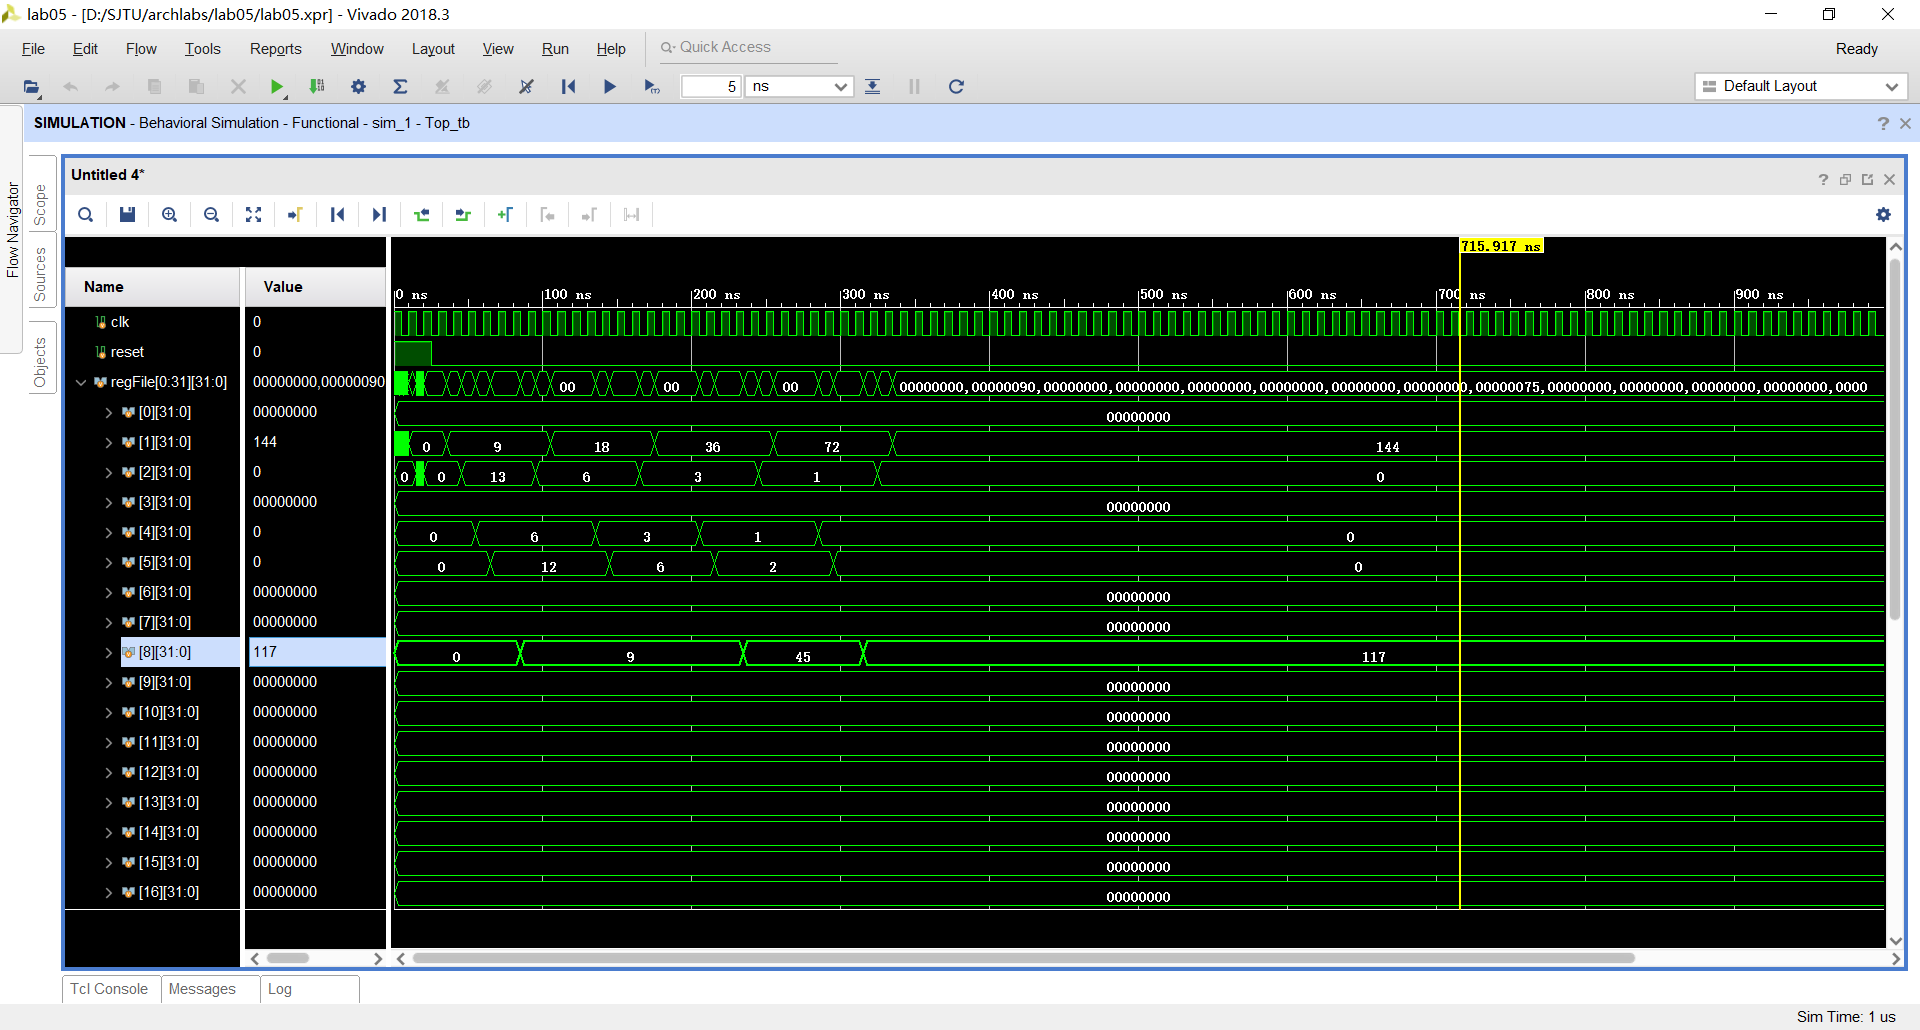
\includegraphics[scale=0.3]{../figure/05/lab05-1.PNG}
    \caption{数据存储器实验结果}\label{fig:1}
\end{figure}

\section{反思与总结}

本次实验实现了一个单周期处理器,总体而言还是比较有挑战性的。在实验过程中为了实现更多的指令,需要对教程上的电路图进行修改,对此我进行了一些比较大胆的尝试,比如更改模块的输入、增加管线等待。通过本次实验,我也对单周期处理器和MIPS指令集有了更为深入的了解。

\end{document}
